\newcommand{\req}[1]{RQ#1}

\section{Evaluation}\label{sec:eval}
%In this section, we show the feasibility of the approach of using declarative
%analysis for multilingual program, and the effectiveness of its
%implementation. More specifically, we set three research questions as follow:

%RQ1) Feasibility: Is it possible to implement a working static analyzer for multilingual program in declarative style?
%
%RQ2) Performance: How is the speed and precision of implemented analyzer, compared to the state-of-the-art analyzer?
%
%RQ3) Usefulness: How practical is the implemented analyzer?

To show the effectiveness of our approach, we evaluate our analyzer with the
following three research questions:
\begin{itemize}
  \item \req{1}: {\it (Feasibility)} Can our tool analyze JNI programs that use
    various JNI inteoperations?

  \item \req{2}: {\it (Performance)} How precise and scalable is our tool for
    real-world JNI program analysis compared to Lee's analyzer~\cite{LeeASE20}?

  \item \req{3}: {\it (Usefulness)} Can our tool analyze the same types of bugs
    the state-of-the-art JNI program analyzers can detect?
\end{itemize}

%To answer RQ1, we tested our implemented analyzer with NativeFlowBench, which
%is a small set of benchmarks manually crafted by authors of JN-SAF[2], with the
%purpose of testing dataflow analyzer for JNI programs. It consists of 23
%android applications featuring various interactions between C and Java, some of
%which contain a malicious code pattern that tries to leak sensitive user data.
%The analyzer should successfully recognize and report those patterns for each
%application, if any. The result showws that our approach is feasible enough,
%in that we could correctly draw call graph, find field access target, and
%find data leaks from the benchmarks.

For \req{1}, we analyze benchmarks in NativeFlowBench~\cite{nativeflowbench,
JN-SAF} using our tool. The benchmarks contain 23 JNI Android applications that
use various JNI interoperations and leak sensitive data from {\it sources} to
{\it sinks} across language boundaries via the interoperations. We also compare
analysis results of our tool to results of Lee's analyzer and JN-SAF. We use
compiled versions of the benchmarks for JN-SAF because it targets compiled JNI
programs, and use source code of the benchmarks for ours and Lee's analyzer.

%To answer RQ2, we applied our analyzer to 42 real-world android applications
%collected from F-Droid[9], a repository for open-source android application.
%These 42 apps are selected by first scannig the apps that feature JNI from the
%repository, and among them, selecting those that we could successfully compile.
%The line number of collected code ragnes from hundreds of lines, to hundreds of
%thousands of lines.  We compared our analyzer with Lee's state-of-the-art JNI
%analyzer[3], and confirmed that our analyzer outperforms in terms of
%scalability and precision.

For \req{2}, we compare analysis results of our tool and Lee's analyzer on 42
real-world JNI Android applications downloaded from F-Droid, a repository of
open-source Android applications~\cite{fdroid}. We first classified
applications of F-Droid into JNI or non-JNI applications. Then, we selected the
42 applications out of all the JNI applications as our analysis targets,
because they are only applications that are compiled without errors.

%To answer RQ2, we applied our analyzer to 42 real-world android applications
%collected from F-Droid[9], a repository for open-source android application.
%These 42 apps are selected by first scannig the apps that feature JNI from the
%repository, and among them, selecting those that we could successfully compile.
%The line number of collected code ragnes from hundreds of lines, to hundreds of
%thousands of lines.  We compared our analyzer with Lee's state-of-the-art JNI
%analyzer[3], and confirmed that our analyzer outperforms in terms of
%scalability and precision.


%To answer RQ1, we tested our implemented analyzer with NativeFlowBench, which
%is a small set of benchmarks manually crafted by authors of JN-SAF[2], with the
%purpose of testing dataflow analyzer for JNI programs. It consists of 23
%android applications featuring various interactions between C and Java, some of
%which contain a malicious code pattern that tries to leak sensitive user data.
%The analyzer should successfully recognize and report those patterns for each
%application, if any. The result showws that our approach is feasible enough,
%in that we could correctly draw call graph, find field access target, and
%find data leaks from the benchmarks.

%tool on benchmarks in NativeFlowBench~\cite{nativeflowbench, JN-SAF}. The
%benchmarks include 23 Android JNI applications that use various JNI
%interoperation features. Because JN-SAF targets compiled JNI programs, we use
%compiled versions of the benchmarks for JN-SAF and source code of the
%benchmarks for Lee's analyzer and our tool. 


%To answer RQ3, we implemented various kinds of bug checkers, introduced in
%previous researches[1][3], on top of our analyzer. We ran our bug checker on
%the 42 applications of F-Droid mentioned above, and detected 33 bugs,
%including \inred{25} newly found bugs.

For \req{3}, we detect JNI interoperation bugs in the 42 real-world Android
applications using our tool. We implemented a checker detecting four types of
bugs on top of our tool using the query language of CodeQL. We chose our target
JNI interoperation bugs as the same as the targets of previous research's
client analyses~\cite{LeeASE20, ILEA}.


\subsection{\req{1}: Feasibility}
\begin{table*}[t]
  \vspace{2mm}
  \caption{The analysis result of NativeFlowBench}
  \label{table:RQ1}
  \vspace*{-1em}
  \centering
  \small
  \begin{tabular}{l|c|c|c|c||l|c|c|c|c}
    \myhead{Benchmark}{Precision}{Dataflow}
    %\myhead{Benchmark}{Lee~\cite{LeeASE20}}{Ours}{Benchmark}{JN-SAF}{Ours}
    icc\_javatonative                   & X & X & O & X & native\_noleak                       & O & O & O & O  \\
    icc\_nativetojava                   & O & O & O & X & native\_noleak\_array                & O & O & X & O  \\
    native\_complexdata                 & O & O & O & O & native\_nosource                     & O & O & O & O  \\
    native\_complexdata\_stringop       & X & X & X & X & native\_pure                         & X & O & O & O  \\
    native\_dynamic\_register\_multiple & O & O & O & O & native\_pure\_direct                 & X & O & O & O  \\
    native\_heap\_modify                & O & O & O & O & native\_pure\_direct\_customized     & X & O & O & O  \\
    native\_leak                        & O & O & O & O & native\_set\_field\_from\_arg        & O & O & O & O  \\
    native\_leak\_array                 & O & O & O & X & native\_set\_field\_from\_arg\_field & O & O & O & O  \\
    native\_leak\_dynamic\_register     & O & O & O & O & native\_set\_field\_from\_native     & O & O & O & O  \\
    native\_method\_overloading         & O & O & O & O & native\_source                       & O & O & O & O  \\
    native\_multiple\_interactions      & O & O & O & O & native\_source\_clean                & O & O & O & O  \\
    native\_multiple\_libraries         & O & O & O & O & \multicolumn{1}{c}{}                 & \multicolumn{1}{c}{} & \multicolumn{1}{c}{} & \multicolumn{1}{c}{} & \multicolumn{1}{c}{}
  \end{tabular}
\end{table*}


Table~\ref{table:RQ1} shows analysis results of our analyzer, Lee's analyzer,
and JN-SAF on 23 benchmarks in NativeFlowBench.  The {\it Benchmark} columns
denote benchmark names, the {\it Precision} columns denote analysis results of
Lee's analyzer and ours, and the {\it Dataflow} columns denote analysis results
of JN-SAF and ours.  Lee's analyzer and JN-SAF have different analysis purposes
each other; Lee's analyzer constructs call graphs of JNI programs, and JN-SAF
detects data leakages from sources to sinks. For fair comparison, we compare
ours and Lee's analyzer for the precision of resolving targets of foreign
function calls, and compare ours and JN-SAF for the data leakage detection
results. We marked each analysis result as success($\bigcirc$) or
failure($\times$). In the precision comparison, an analysis succeeds if
it precisely resolves targets of all foreign function calls between Java and C,
and it fails otherwise. In the dataflow comparison, an analysis succeeds
if it reports all data leakages correctly without false positivies or
negatives.


%of columns denote whether the analysis result for corresponding benchmark is
%correct(O), incorrect(X), or not available(-) in terms of two criteria for each
%of the analyzers. For the "Precision" columns we call the analysis result is
%correct if every function call (call from Java to C, call from C to Java)
%target and field access (field read from C to Java, field write from C to Java)
%target is precisely determined. For "Dataflow" columns, it's considered correct
%if every data leak is reported correctly without false positives nor false
%negatives. 

%For precision, we compare our result with Lee's analyzer, since JN-SAF does not
%provide the function call / field access target information. Except for two
%benchmarks, our analyzer could correctly determine all targets for function
%calls and field access correctly.  One of two exception benchmarks was
%\textit{icc\_java\_to\_native}, which reported two more suprious call edges for
%a function call of android library function from C to Java. The other exception
%was \textit{native\_complexdata\_stringop}, where string manipulation functions
%such as strcpy or strcat from C standard library were used to create the string
%value that indicates the target field's name. Since the inner-flow analysis
%could not properly model these string manipulation functions, analyzer could
%not correctly determine the field access target. Still, the overall result is
%superior to the Lee's, which could not precisely analyze the 4 additional
%benchmarks.

In the precision comparison, our tool successfully analyzed 21 out of 23
benchmarks, while Lee's analyzer failed in three more benchmarks than ours. We
manually confirmed that the two common failures of Lee's and ours are
originated from built-in structs and functions in C; {\it
icc\_java\_to\_native} stores Java class information in the Android built-in
structure {\tt android\_app} and {\it native\_complexdata\_stringop} generates
a Java field name by concatenating two string values via the {\tt strcat}
built-in function. Because ours and Lee's analyzer do not handle such built-in
structs and functions, they failed to analyze the two benchmarks.  Lee's
analyzer failed to analyze the three more benchmarks due to native entry points
or the benchmarks~\cite{nativeactivity}. FlowDroid~\cite{Flowdroid} used by
Lee's analyzer performs the whole-program analysis from Android entry points.
Because the benchmarks have entry points only in C differently from monolingual
Android applications, FlowDroid cannot find entries from which its analysis
starts.  Contrary to Lee's analyzer, our tool performs the query-based
analysis, which can resolve targets of foreign function calls regardless of
program entries.


In the dataflow comparison, our tool found data leakages correctly in 19
benchmarks but reported false alarms for four benchmarks, while JN-SAF analyzes
21 benchmarks correctly. The one common failure is originated from the string
concatenation as we described. {\it icc\_javatonative} and {\it
icc\_nativetojava} leak data via the Android inter-component communication that
is beyond the scope of this paper. The remaining two different failures of ours
and JN-SAF come from their array analysis policies. {\it native\_leak\_array}
stores sensitive data in an array, and then retreives the data from the array
and leaks it. On the other hand, {\it native\_noleak\_array} stores sensitive
data in an array as well, but retrieves another element from the array and uses
it. Because distinguishing different index of an array is challenging, JN-SAF
tracks every value retrieved from an array if the array contains sensitive
data. Such over-approaximation enables JN-SAF to analyze {\it
native\_leak\_array} correctly, but introduce false alarm on {\it
native\_noleak\_array} at the same time. In contrast, because CodeQL does not
track dataflows depending on arrays by default, our tool does not report false
alarm on {\it native\_noleak\_array} but cannot find the data leakage in {\it
native\_leak\_array}.


\subsection{RQ2: Performance}
\begin{table*}[t]
  \vspace{2mm}
  \caption{The analysis result for F-Droid applications}
  \label{table:RQ2}
  \vspace*{-1em}
  \centering
  \small
  \begin{tabular}{l||r|r|r|r|r||r|r|r||r|r|r}
    \multirow{3}{*}{\textbf{Application}} & \multicolumn{5}{c||}{\textbf{Time (sec.)}} & \multicolumn{3}{c||}{\multirow{2}{*}{\textbf{C->Java Function Call}}} & \multicolumn{3}{c}{\multirow{2}{*}{\textbf{C->Java Field Access}}} \\\hhline{~||-----||~~~||~~~}
    & \multicolumn{3}{c|}{\textbf{DB Creation}} & \multicolumn{1}{c|}{\multirow{2}{*}{\textbf{Query}}} & \multicolumn{1}{c||}{\multirow{2}{*}{\textbf{Total}}} & \multicolumn{3}{c||}{} & \multicolumn{3}{c}{} \\\hhline{~||---~|~||------}
    & \multicolumn{1}{c|}{\textbf{C}} & \multicolumn{1}{c|}{\textbf{Java}} & \multicolumn{1}{c|}{\textbf{Merged}} & \multicolumn{1}{c|}{} & \multicolumn{1}{c||}{} & \multicolumn{1}{c|}{\textbf{\# Precise}} & \multicolumn{1}{c|}{\textbf{\# Resolved}} & \multicolumn{1}{c||}{\textbf{Total}} & \multicolumn{1}{c|}{\textbf{\# Precise}} & \multicolumn{1}{c|}{\textbf{\# Resolved}} & \multicolumn{1}{l}{\textbf{Total}}  \\\hhline{=#*{4}{=|}=#=|=|=#=|=|=}
  Agram                  & 2.538                 & 5.002                    & 3.643                      & 6.829                                      & 18.012                                  & 0                           & 0                            & 2                         & 4                           & 4                            & 4                          \\
  AndIodine              & 2.805                 & 8.237                    & 3.989                      & 8.114                                      & 23.145                                  & 1                           & 1                            & 1                         & 0                           & 0                            & 0                          \\
  APV PDF Viewer         & 56.496                & 9.252                    & 23.349                     & 35.688                                     & 124.785                                 & 4                           & 4                            & 4                         & 15                          & 15                           & 16                         \\
  CommonsLab             & 23.176                & 24.139                   & 14.149                     & 20.554                                     & 82.018                                  & 4                           & 5                            & 5                         & 0                           & 0                            & 0                          \\
  CrossWords             & 29.754                & 21.663                   & 23.276                     & 29.106                                     & 103.799                                 & 68                          & 68                           & 70                        & 9                           & 10                           & 14                         \\
  Document Viewer        & 180.71                & 20.292                   & 56.743                     & 75.934                                     & 333.679                                 & 6                           & 6                            & 6                         & 23                          & 23                           & 24                         \\
  DroidZebra             & 17.774                & 7.141                    & 5.817                      & 12.608                                     & 43.34                                   & 4                           & 5                            & 5                         & 0                           & 0                            & 0                          \\
  FBReader               & 85.398                & 27.114                   & 36.36                      & 30.072                                     & 178.944                                 & 0                           & 0                            & 0                         & 0                           & 0                            & 1                          \\
  Fwknop2                & 11.834                & 11.488                   & 7.395                      & 10.446                                     & 41.163                                  & 0                           & 0                            & 0                         & 0                           & 13                           & 13                         \\
  Graph 89               & 72.609                & 8.47                     & 41.465                     & 598.645                                    & 721.189                                 & 1                           & 1                            & 1                         & 0                           & 0                            & 0                          \\
  Irssi ConnectBot       & 1.284                 & 12.32                    & 6.048                      & 11.196                                     & 30.848                                  & 1                           & 1                            & 1                         & 0                           & 0                            & 2                          \\
  Lumicall               & 40.486                & 13.102                   & 17.328                     & 27.104                                     & 98.02                                   & 4                           & 4                            & 4                         & 2                           & 2                            & 13                         \\
  Navit                  & 26.761                & 17.741                   & 54.751                     & 46.264                                     & 145.517                                 & 16                          & 22                           & 55                        & 0                           & 0                            & 0                          \\
  NetGuard               & 14.958                & 16.925                   & 9.988                      & 12.716                                     & 54.587                                  & 0                           & 9                            & 9                         & 3                           & 27                           & 27                         \\
  Overchan               & 1.727                 & 22.043                   & 8.772                      & 15.143                                     & 47.685                                  & 1                           & 2                            & 4                         & 0                           & 0                            & 1                          \\
  Plumble                & 28.501                & 12.365                   & 16.335                     & 29.253                                     & 86.454                                  & 0                           & 0                            & 0                         & 610                         & 610                          & 610                        \\
  PrBoom                 & 48.312                & 5.469                    & 21.601                     & 32.001                                     & 107.383                                 & 7                           & 7                            & 15                        & 0                           & 0                            & 0                          \\
  Rtl-sdr driver         & 18.797                & 16.984                   & 9.623                      & 11.751                                     & 57.155                                  & 2                           & 2                            & 2                         & 0                           & 0                            & 0                          \\
  Sipdroid               & 20.267                & 11.864                   & 10.961                     & 18.577                                     & 61.669                                  & 2                           & 2                            & 2                         & 2                           & 2                            & 16                         \\
  Son of Hunky Punk      & 40.266                & 14.947                   & 20.582                     & 31.102                                     & 106.897                                 & 50                          & 50                           & 52                        & 10                          & 10                           & 10                         \\
  Taps Of Fire           & 3.566                 & 7.521                    & 4.453                      & 8.145                                      & 23.685                                  & 0                           & 0                            & 0                         & 2                           & 2                            & 2                          \\
  Tileless Map           & 273.993               & 187.099                  & 118.557                    & 146.806                                    & 726.455                                 & 50                          & 58                           & 59                        & 3                           & 4                            & 5                          \\
  Timidity AE            & 23.417                & 11.718                   & 13.03                      & 28.452                                     & 76.617                                  & 16                          & 16                           & 16                        & 0                           & 0                            & 0                          \\
  Tux Paint              & 256.126               & 120.831                  & 161.906                    & 184.591                                    & 723.454                                 & 80                          & 83                           & 89                        & 4                           & 4                            & 6                          \\
  VotAR                  & 1.515                 & 5.189                    & 3.569                      & 6.532                                      & 16.805                                  & 1                           & 1                            & 2                         & 3                           & 3                            & 3                          \\\hhline{=#*{4}{=}=#=|=|=#=|=|=}
    \textbf{Total}       & \multicolumn{1}{r}{}  & \multicolumn{1}{r}{}     & \multicolumn{1}{r}{}       & \multicolumn{1}{r}{}                       & \multicolumn{1}{r||}{}                    & 318                         & 347                          & 404                       & 690                         & 729                          & 767
  \end{tabular}
\end{table*}

Table~\ref{table:RQ2} shows analysis results of our tool on real-world Android
JNI applications. Out of 42 applications we analyzed, we summarize analysis
results of 25 applications that have interoperation from C to Java.\footnote{We
list full analysis results up in our supplementary material.} \inred{The first column
denotes application names, the second to fourth columns show database creation
time for C code, Java code, and ...}

%The "time" column denotes the time for creating database and evaluating query.
%The average time for creating DB was 103.8 seconds, and average time for
%evaluating query was 57.5 seconds, making the average of total analysis time
%161.3 seconds. The longest time it took to analyze was 726.5 seconds for
%analyzing \inred{??} lines of codes, which is about 12 minutes.

%The "precision" columns denotes the precision of dispatching function call
%target, and field access target.  "Precise" means exactly one target was found,
%and resolved means at least one target was found. For the function call from C to Java,
%\inred{???}\% of function calls were resolved, and \inred{???}\% of functions calls
%were precisely resolved. For the field access, \inred{???}\% of field accesses (both
%read and write) were resolved, and \inred{???}\% of field access were precisely resolved.
%Compared to the precision result of the state-of-the-art analyzer, our implementation
%showed higher precision.

Our analyzer resolved 1076 out of 1171 (92\%) foreign function calls, including
347 out of 404 (86\%) C-to-Java method calls and 729 out of 767 (95\%)
C-to-Java field accesses. In addition, 1008 (86\%) resolved foreign function
calls are precies. The results show that our tool resolves more foreign
function calls even precisley than Lee's analyzer that \inred{...} on the same
dataset. Our analyzer failed to resolve 95 (8\%) foreign function calls because
of complex language semantics such as arrays and function pointers. Because
CodeQL does not track dataflows depending on C function pointers as well as
arrays we descibed, our analyzer failed to analyze method or field IDs required
to resolve the foreign function calls.

\begin{figure}[t]
  \centering
  \vspace{2mm}
  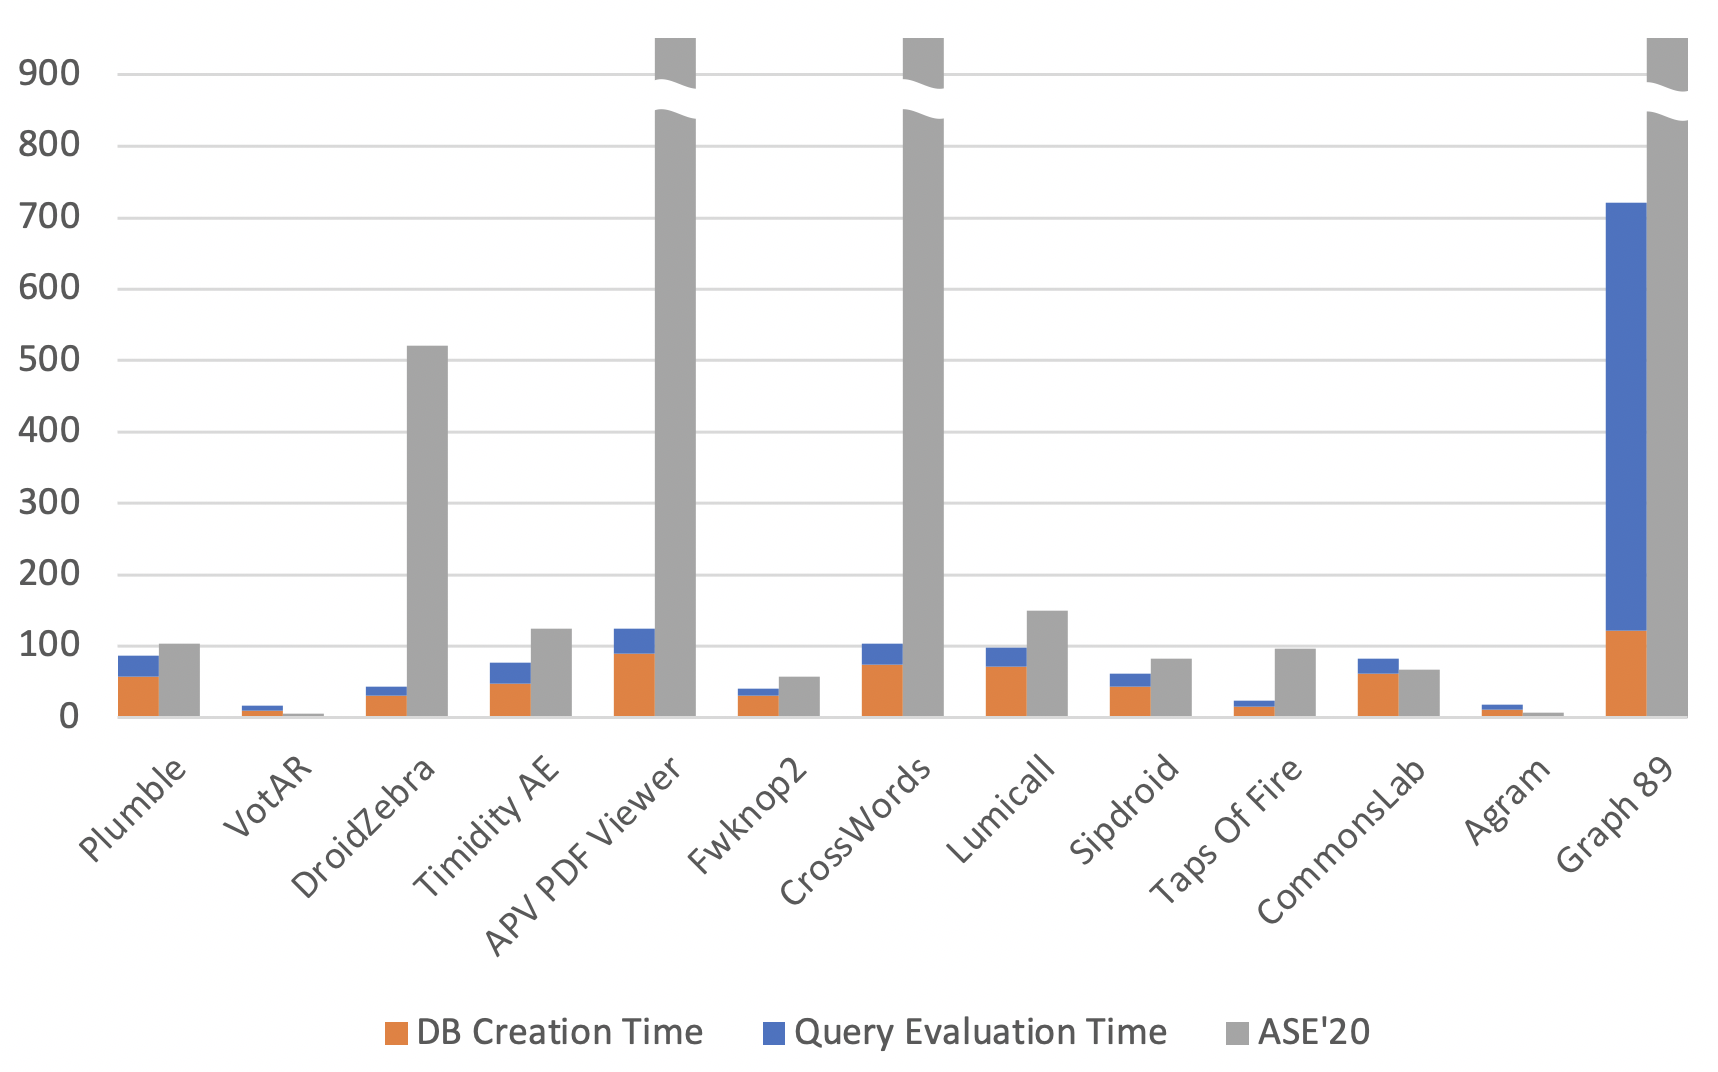
\includegraphics[width=0.5\textwidth]{img/graph}
  \vspace*{-1.5em}
  \caption{Speedup}
  \label{fig:graph}
\vspace*{-.5em}
\end{figure}

Our analyzer is scalable even for large-scale programs as well. The analysis
time was 161.3 seconds on average for each application, including 103.8 seconds
for the DB creation and 57.5 seconds for the query processing. The DB creation
usually took more time than the query processing except for {\it Graph 89}, and
the DB creation time was almost linear to the size of code. Our analyzer took
about 12 minutes at most to analyze {\it Tileless Map} having about one million
lines of code. Figure~\ref{fig:graph} visualizes analysis time of our analyzer
compared to Lee's analyzer. \inred{describe the comparison result...}  Note
that once we create database for a program, we can evaluate multiple queries on
it without re-creation to gain various analysis results of the program.


%Applications that do not have interaction form C to Java is ommitted from the
%table, and we summarize the result for 25 of 42 apps, which contains call to
%Java method or access to Java field access from C.\footnote{The full list of data
%is submitted to supplementary material.}

%The "time" column denotes the time for creating database and evaluating query.
%The average time for creating DB was 103.8 seconds, and average time for
%evaluating query was 57.5 seconds, making the average of total analysis time
%161.3 seconds. The longest time it took to analyze was 726.5 seconds for
%analyzing \inred{??} lines of codes, which is about 12 minutes.

%In conclusion, considering that our analyzer could successfully analyze the
%benchmark applications with higher precision in significantly shorter time
%compared to the stat-of-the-art analyzer, we conclude that our implementation
%has competitive performance.

\subsection{RQ3: Usefulness}
\begin{table}[t]
  \vspace{2mm}
  \caption{Bug detection results of real-world Android JNI apps}
  \label{table:RQ3}
  \vspace*{-1em}
  \centering
  \small
\renewcommand{\arraystretch}{.9}
  \begin{tabular}{l||r|r|r|r|r} 
    \multirow{4}{*}{\textbf{Application}} &
                                            \multicolumn{5}{c}{\textbf{Bug Kind}} \\\hhline{~||-----}
                                          & \multicolumn{2}{c|}{\textbf{Null}}   & \multicolumn{1}{c|}{\textbf{Missing}} & \multicolumn{1}{c|}{\textbf{Type}} & \multicolumn{1}{c}{\textbf{Wrong}} \\\hhline{~||~|~|~|~|~}
                                          & \multicolumn{2}{c|}{\textbf{Deref.}} & \multicolumn{1}{c|}{\textbf{Fun}} & \multicolumn{1}{c|}{\textbf{Mis.}} & \multicolumn{1}{c}{\textbf{\textbf{Sig.}}}  \\\hhline{~||-|-|-|-|-}
                                          & \multicolumn{1}{c|}{\textbf{\# TP}}   & \multicolumn{1}{c|}{\textbf{\# FP}} & \multicolumn{1}{c|}{\textbf{\# TP}} & \multicolumn{1}{c|}{\textbf{\# TP}} & \multicolumn{1}{c}{\textbf{\textbf{\# TP}}}  \\\hhline{=#=|=|=|=|=}

    APV PDF Viewer    & 0 & 1 & 0 & \cellcolor{\succcolor}2 & 0 \\ 
    CrossWords        & \cellcolor{\succcolor}3 & 1 & 0 & 0 & 0 \\ 
    Document Viewer   & 0 & 0 & 0 & \cellcolor{\succcolor}1 & 0 \\ 
    DroidZebra        & 0 & 1 & 0 & 0 & 0 \\ 
    FBReader          & 0 & 9 & 0 & \cellcolor{\succcolor}1 & 0 \\ 
    Graph 89          & \cellcolor{\succcolor}1 & 0 & 0 & \cellcolor{\succcolor}3 & 0 \\ 
    KeePassDroid      & \cellcolor{\succcolor}1 & 0 & 0 & 0 & 0 \\
    Lumicall          & 0 & 0 & \cellcolor{\succcolor}3 & 0 & 0 \\ 
    Lunary            & 0 & 1 & 0 & 0 & 0 \\
    Ministro          & 0 & 0 & 0 & \cellcolor{\succcolor}1 & 0 \\ 
    Navit             & 0 & 0 & 0 & \cellcolor{\succcolor}3 & 0 \\ 
    Hacker's Keyboard & 0 & 1 & 0 & 0 & 0 \\ 
    NetGuard          & 0 & 1 & 0 & 0 & 0 \\ 
    ObscuraCam        & 0 & 0 & \cellcolor{\succcolor}2 & 0 & 0 \\ 
    PrBoom            & 0 & 0 & 0 & 0 & \cellcolor{\succcolor}1 \\
    Sipdroid          & 0 & 0 & \cellcolor{\succcolor}4 & 0 & 0 \\ 
    Tileless Map      & 0 & 2 & 0 & \cellcolor{\succcolor}3 & 0 \\ 
    Tux Paint         & 0 & 4 & 0 & \cellcolor{\succcolor}3 & 0 \\ 
    VotAR             & 0 & 0 & 0 & 0 & \cellcolor{\succcolor}1 \\\hhline{=#=|=|=|=|=}
    \textbf{Total}    & 5 & 21 & 9 & 17 & 2 \\
  \end{tabular}
\end{table}

Table~\ref{table:RQ3} shows the list of bugs and security vulnerabilities we could detect.
The first bug is the null dereference bug[1][9], which detects the dereference of
Java's null value in C, without proper nullity checking logic. Rest of three
bugs are related to mistake in using interaction, which are described in
previous research[2]. "Missing fun" denotes the case where C function is
missing even if it is called from java. "Type mismatch" denotes the case where
the declaration of native function in Java has different return type or
parameter type with its actual definition in C.  "Wrong signature" denotes the
case where "GetMethodID" uses wrong signature for the java method. The
number in each cell denotes the number of alarms, and the number in the
parenthesis denotes the number of false alarm, if any.

\begin{figure}[t]
  \centering
  \vspace{2mm}
  \begin{subfigure}[t]{0.5\textwidth}
    \begin{lstlisting}[style=cpp,xleftmargin=2.5em]
//EmulatorActivity.java
String tmp = null;
String folder = Util.GetInternalAppStorage(activity);

if (folder != null) {
  tmp = folder + "tmp";
  Util.CreateDirectory(tmp);
}

EmulatorActivity.nativeInitGraph89(..., tmp);

//wrappercommonjni.c
void Java_..._nativeInitGraph89(..., jstring tmp_dir) {
   (*env)->GetStringUTFChars(env, tmp_dir, 0);
   ...
}
    \end{lstlisting}
    \vspace*{-.5em}
    \caption{Null dereference}
    \label{fig:bug1}
  \end{subfigure}
  \begin{subfigure}[t]{0.5\textwidth}
    \begin{lstlisting}[style=cpp,xleftmargin=2.5em]
//JpegRedaction.java
package org.witness.obscuracam.photo.jpegredaction;

public class JpegRedaction {
  private native void redactRegions(...);
  ...
}

//JpegRedaction.cpp
void
Java_org_witness_securesmartcam_jpegredaction_ JpegRedaction_redactRegions(...) {
  ...
}
    \end{lstlisting}
    \vspace*{-.5em}
    \caption{Missing Fun}
    \label{fig:bug2}
  \end{subfigure}
  \begin{subfigure}[t]{0.5\textwidth}
    \begin{lstlisting}[style=cpp,xleftmargin=2.5em]
//MuPdfPage.java
private native static List<PageTextBox> search(...);

//mupdfdroidbridge.c
jobjectArray Java_..._search(...){
   ...
 }
    \end{lstlisting}
    \vspace*{-.5em}
    \caption{Type Mismatch}
    \label{fig:bug3}
  \end{subfigure}
  \begin{subfigure}[t]{0.5\textwidth}
    \begin{lstlisting}[style=cpp,xleftmargin=2.5em]
//PrBoomActivity.java
void OnMessage(String text);
void OnInfoMessage(String msg, int displayType);

//jni_doom.h
#define CB_CLASS_MSG_SIG  "(Ljava/lang/String;I)V"
#define CB_CLASS_INFMSG_SIG  "(Ljava/lang/String;I)V"

//jni_doom.c
mSendStr = (*env)->GetMethodID(env, jNativesCls, "OnMessage", CB_CLASS_MSG_SIG);

    \end{lstlisting}
    \vspace*{-.5em}
    \caption{Wrong Signature}
    \label{fig:bug3}
  \end{subfigure}
  \vspace*{-.5em}
  \caption{Real excerpt of examples of bugs}
  \label{fig:bugs}
\end{figure}

We demonstrate some interesting bugs we found in our benchmark with actual minified examples above
for each kind.

First example denotes null dereference bug. A null is stored in variable tmp, and
it is updated into non-null value under certain condition. However, tmp is passed
to a C function even if it is still null, and it is dereferenced there
without proper check.

Second example denotes a bug where C function is missing. The name for target C
function is decided with convention, and the java package's name is used
for deciding the name. It seems that package name is changed during development,
but the function name in the C source code was not changed respectively, resulting
in missing function bug.

In third example, the return type of the function is List, which is an object.
However, in C, the return type of the function is defined as "jarray", which
should be used for array, not object.

In the final example, it demonstrates the case where wrong signature is used
for dispatching java method from C, using "GetMethodID" function. An interesting
point is that, the signatures were defined in C macro, and the wrong signature
was the same as the next one.

We manually inspected the source code if the reported alarms are false positive
or not. No false positives were found for latter three kinds of bugs.  There
were some false positive for the first bug, the null dereference bug. The
reason for these false positives were mainly due to, again, imprecise
intra-language dataflow. For example, the analyzer could not handle the case
where a variable is reassigned to a non-null value in a different branch or a
different function, resulting in giving the false positive that null value can
be dereferenced.

In summary, we can conclude that our analyzer is practical and useful enough,
in that we could find previously unknown bugs/security vulnerabilities using
our analyzer.
